\documentclass[11pt]{article}
\usepackage{amsmath}
\usepackage{amsfonts}
\usepackage{graphicx}
\usepackage{hyperref}
\usepackage{geometry}

% Page setup
\geometry{a4paper, margin=1in}

\title{Numerical Investigation of a Magneto-Elastic Beam System}
\author{}
\date{}

\begin{document}

\maketitle

\section*{Introduction}
This document presents a numerical investigation of the dynamics of a magneto-elastic beam, modeled as a Hamiltonian system. The dynamics are governed by a Hamiltonian function that captures the kinetic and potential energy contributions, leading to a system of first-order differential equations. We solve these equations numerically using the fourth-order Runge-Kutta method and analyze the results through a phase portrait.

\section*{The Hamiltonian System}
The Hamiltonian for the magneto-elastic beam is given by:
\[
H(q, p) = \frac{1}{2m} p^2 - \frac{1}{2} \beta^2 q^2 + \frac{1}{4} q^4,
\]
where:
\begin{itemize}
    \item \( q \): Displacement of the beam from the line of symmetry.
    \item \( p \): Momentum conjugate to \( q \).
    \item \( m \): Mass of the system.
    \item \( \beta \): Parameter controlling the strength of the quadratic potential.
\end{itemize}

The equations of motion derived from the Hamiltonian are:
\[
\dot{q} = \frac{\partial H}{\partial p} = \frac{p}{m}, \quad
\dot{p} = -\frac{\partial H}{\partial q} = \beta^2 q - q^3.
\]

\section*{Numerical Scheme}
The system of first-order differential equations is solved using the fourth-order Runge-Kutta (RK4) method, which approximates the solution at each time step by:
\[
y_{n+1} = y_n + \frac{\Delta t}{6}(k_1 + 2k_2 + 2k_3 + k_4),
\]
where:
\[
k_1 = f(t_n, y_n), \quad
k_2 = f\left(t_n + \frac{\Delta t}{2}, y_n + \frac{\Delta t}{2}k_1\right),
\]
\[
k_3 = f\left(t_n + \frac{\Delta t}{2}, y_n + \frac{\Delta t}{2}k_2\right), \quad
k_4 = f(t_n + \Delta t, y_n + \Delta t k_3).
\]

\section*{Results}
The phase portrait is constructed by numerically integrating the equations of motion for a grid of initial conditions in the \( (q, p) \)-plane. Each trajectory represents the evolution of the system's state in the phase space, revealing the dynamical behavior under the influence of the potential energy.

\begin{figure}[h!]
    \centering
    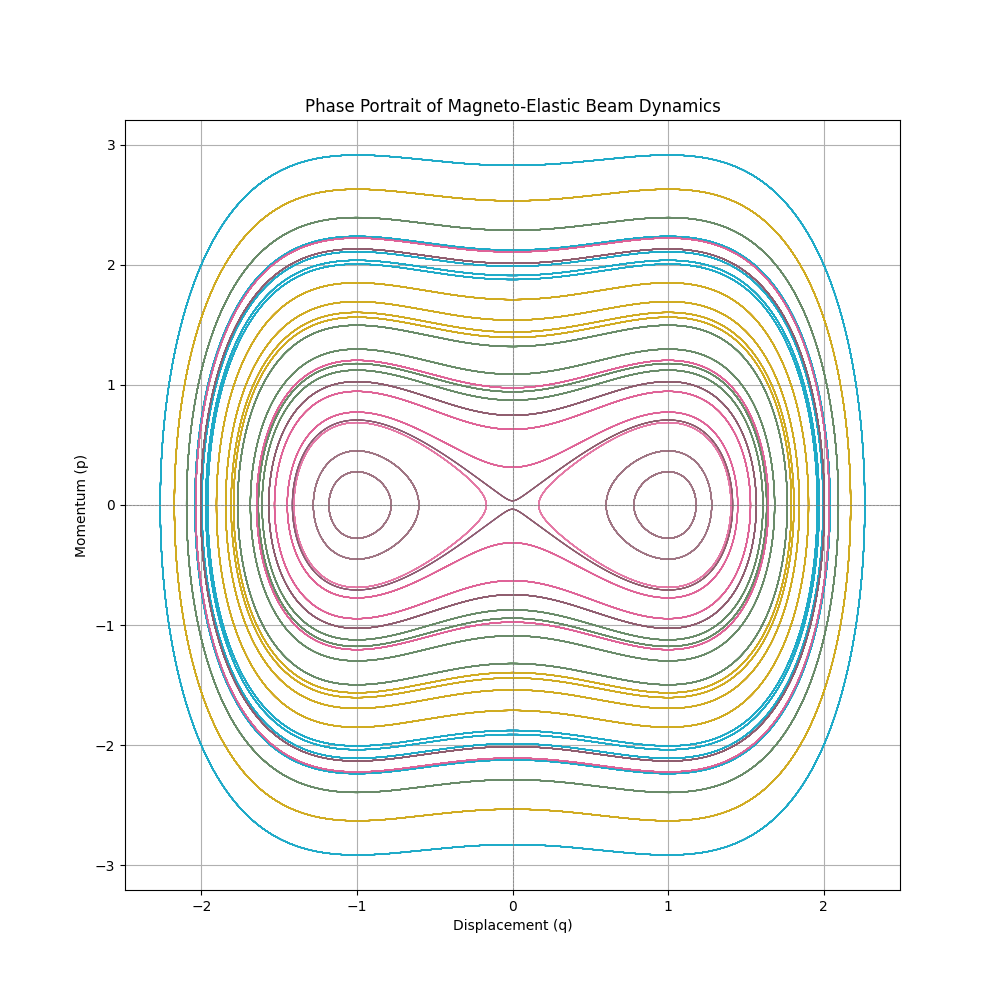
\includegraphics[width=\textwidth]{magneto-elastic_Beam_phase_Portrait.png}
    \caption{Phase portrait of the magneto-elastic beam system. Each curve represents the trajectory of the system in the \( (q, p) \)-plane for a given initial condition.}
    \label{fig:phase_portrait}
\end{figure}

\section*{Conclusion}
The numerical results provide insights into the dynamics of the magneto-elastic beam. The trajectories in the phase space highlight the periodic motion of the system and the effect of nonlinearities introduced by the quartic potential term. Future work can explore bifurcations by varying the parameter \( \beta \) or adding external forcing to the system.

\section*{Poincaré Map}
The Poincaré map is a powerful tool in the analysis of dynamical systems, particularly those subjected to periodic forcing. It provides a discrete representation of a continuous-time dynamical system by sampling the system state at regular intervals, typically synchronized with the period of the external forcing.

\subsection*{Definition}
Consider a dynamical system described by the Duffing equation:
\[
\ddot{x} + b \dot{x} - \beta x + x^3 = F \cos(\omega t),
\]
where \(b\) is the damping coefficient, \(\beta\) determines the linear stiffness, and \(F\) and \(\omega\) are the amplitude and frequency of the external forcing, respectively. The Poincaré map is constructed by observing the state of the system \((x, \dot{x})\) at discrete times:
\[
t_n = t_0 + nT, \quad T = \frac{2\pi}{\omega}, \quad n \in \mathbb{Z},
\]
where \(T\) is the period of the forcing function.

\subsection*{Purpose}
The Poincaré map reduces the continuous-time evolution of the system to a discrete map in the phase space. It captures the system's long-term behavior, highlighting:
\begin{itemize}
    \item Periodic orbits: Represented as fixed points or closed loops in the map.
    \item Chaotic attractors: Appearing as a fractal-like collection of points.
    \item Stability transitions: Observed through bifurcations in the map's structure.
\end{itemize}

\subsection*{Methodology}
To construct the Poincaré map:
\begin{enumerate}
    \item Numerically integrate the Duffing equation over a time interval much longer than the forcing period \(T\).
    \item Record the system's state \((x, \dot{x})\) at each multiple of \(T\).
    \item Plot the sampled points \((x, \dot{x})\) to reveal the map.
\end{enumerate}

\subsection*{Results Interpretation}
The Poincaré map can reveal a range of dynamical behaviors:
\begin{itemize}
    \item For small forcing amplitudes \(F\), the system exhibits periodic motion, visible as a few distinct points in the map.
    \item As \(F\) increases, period-doubling cascades may occur, leading to chaotic dynamics.
    \item In the chaotic regime, the map forms a strange attractor, reflecting the system's sensitivity to initial conditions.
\end{itemize}

The Poincaré map serves as a compact and insightful representation of the complex dynamics of the Duffing equation, aiding in the understanding of periodic and chaotic regimes.

\section*{Combined Poincaré Map and Phase Portrait}
In addition to the Poincaré map, we also include the associated phase portrait of the Duffing equation for a comprehensive visualization of the system's dynamics. This section describes how the plots are generated and their significance in analyzing the Duffing oscillator.

\subsection*{Phase Portrait}
The phase portrait provides a continuous view of the system's trajectory in the \((x, \dot{x})\)-plane, representing the displacement (\(x\)) and velocity (\(\dot{x}\)) of the system over time. It highlights:
\begin{itemize}
    \item The continuous evolution of the system in phase space.
    \item The presence of attractors, limit cycles, and chaotic trajectories.
\end{itemize}

For the Duffing equation:
\[
\ddot{x} + b \dot{x} - \beta x + x^3 = F \cos(\omega t),
\]
the phase portrait is constructed by numerically integrating the system using the Runge-Kutta method and plotting the trajectory over time in the \((x, \dot{x})\)-plane.

\subsection*{Poincaré Map}
The Poincaré map is a discrete representation of the system's dynamics, sampling the state \((x, \dot{x})\) at regular intervals synchronized with the period of the external forcing \(T = 2\pi/\omega\). It highlights:
\begin{itemize}
    \item Periodic orbits, which appear as a small set of discrete points.
    \item Chaotic attractors, which manifest as fractal-like collections of points.
\end{itemize}

\subsection*{Combined Visualization}
By plotting the phase portrait and Poincaré map side by side, we gain a deeper understanding of the system's behavior:
\begin{itemize}
    \item The phase portrait provides a continuous-time perspective.
    \item The Poincaré map simplifies the visualization by reducing the system to a discrete map, making periodicity and chaos easier to identify.
\end{itemize}

\subsection*{Results}
Figure~\ref{fig:duffing_phase_and_poincare} shows the combined plots for the Duffing equation with the following parameters:
\begin{itemize}
    \item Damping coefficient: \(b = 0.2\).
    \item Linear stiffness: \(\beta = 1.0\).
    \item Forcing amplitude: \(F = 0.3\).
    \item Forcing frequency: \(\omega = 1.0\).
    \item Initial conditions: \(x_0 = 0.1\), \(\dot{x}_0 = 0.0\).
\end{itemize}

\begin{figure}[h!]
    \centering
    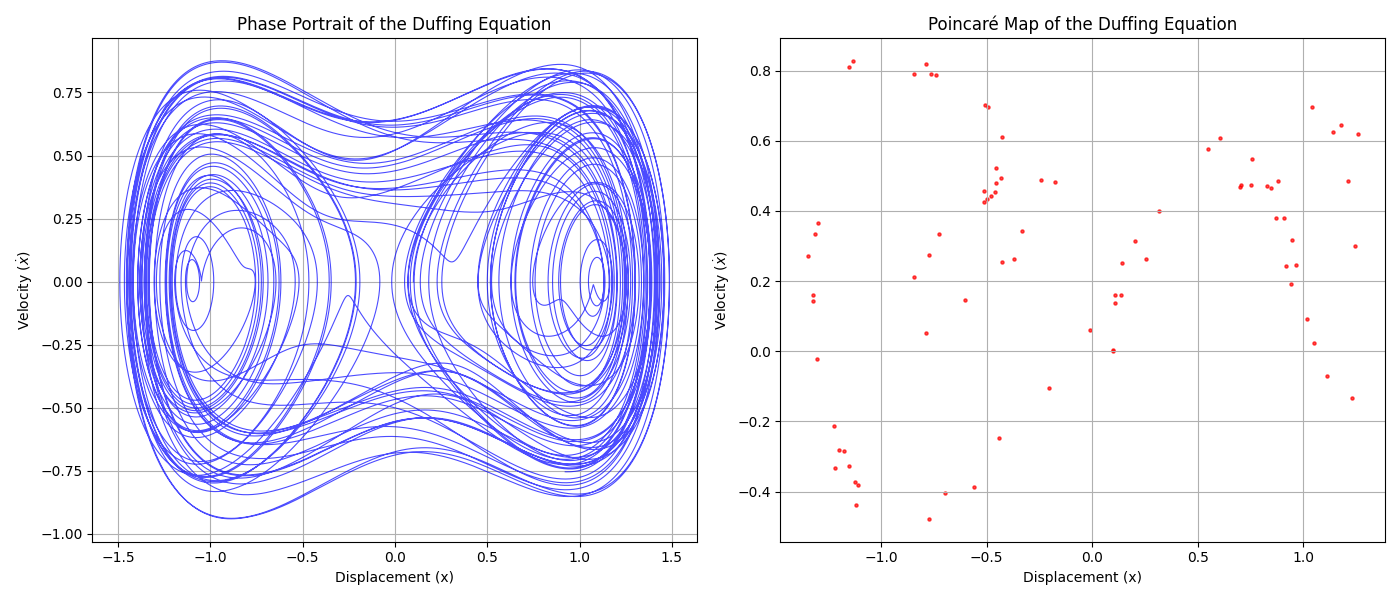
\includegraphics[width=\textwidth]{duffing_phase_and_poincare.png}
    \caption{Combined Phase Portrait and Poincaré Map of the Duffing Equation. The left plot shows the phase portrait, while the right plot depicts the Poincaré map.}
    \label{fig:duffing_phase_and_poincare}
\end{figure}

\subsection*{Conclusion}
The combined visualization offers a detailed perspective on the dynamics of the Duffing equation. The phase portrait highlights the continuous-time trajectories, while the Poincaré map reveals discrete structures such as periodic orbits and chaotic attractors, providing insights into the system's stability and transitions to chaos.

\section*{Unforced Dynamics and Bifurcation Analysis}
The unforced Duffing equation is represented as:
\[
\ddot{x} + b \dot{x} - \beta x + x^3 = 0,
\]
where \(b\) is the damping coefficient, and \(\beta\) determines the linear stiffness. In the absence of external forcing (\(F = 0\)), the dynamics depend on the parameter \(\beta\), leading to a pitchfork bifurcation as \(\beta\) crosses zero.

\subsection*{Simulation and Results}
We simulated the unforced Duffing equation for three values of \(\beta\):
\begin{itemize}
    \item \(\beta < 0\): The system has a single stable equilibrium at \(x = 0\).
    \item \(\beta = 0\): The system undergoes a pitchfork bifurcation, with \(x = 0\) transitioning from stable to unstable.
    \item \(\beta > 0\): The system has two stable equilibria at \(x = \pm\sqrt{\beta}\) and one unstable equilibrium at \(x = 0\).
\end{itemize}

\begin{figure}[h!]
    \centering
    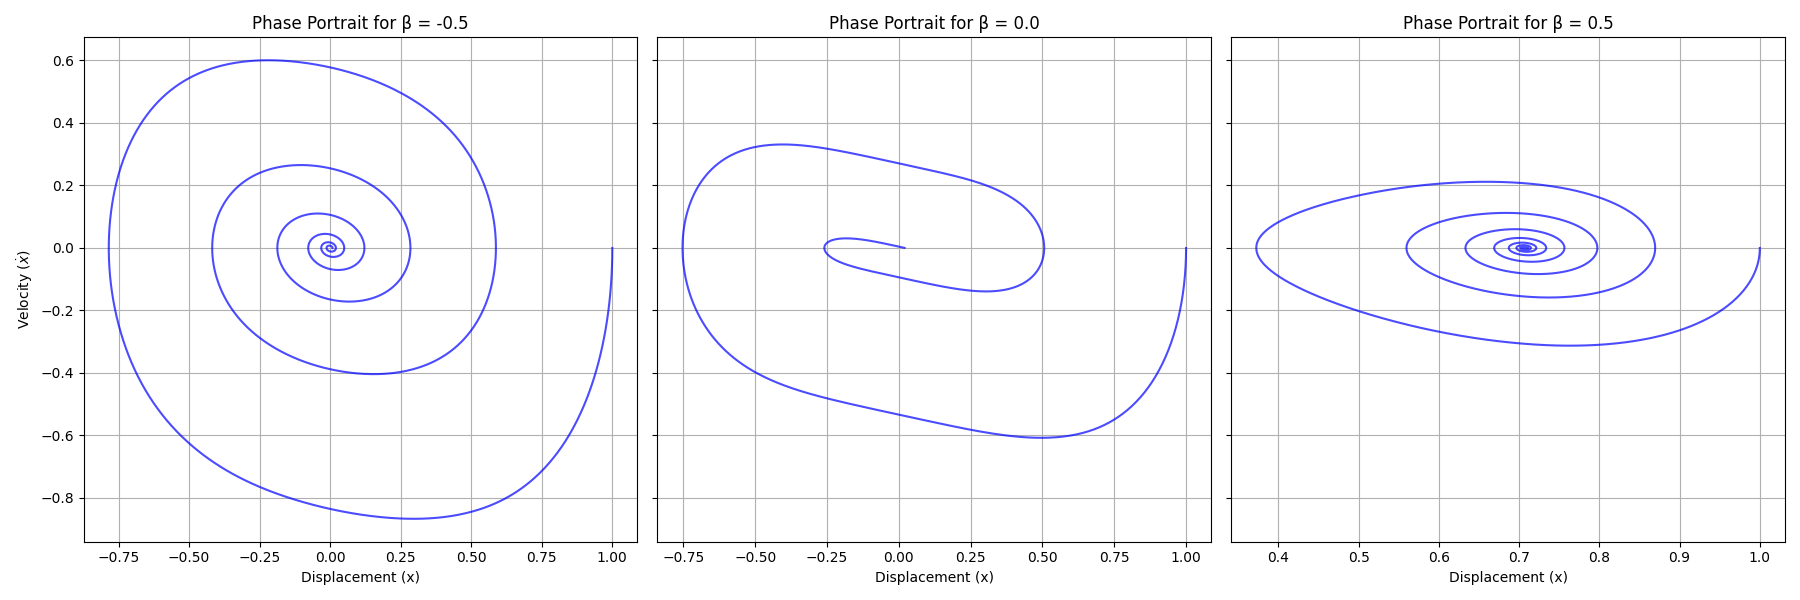
\includegraphics[width=\textwidth]{unforced_duffing_phase_portraits.png}
    \caption{Phase portraits of the unforced Duffing equation for different values of \(\beta\). The plots demonstrate the pitchfork bifurcation as \(\beta\) crosses zero.}
    \label{fig:unforced_phase_portraits}
\end{figure}

\subsection*{Interpretation}
The phase portraits reveal the system's transitions:
\begin{itemize}
    \item For \(\beta < 0\), the system's trajectories converge to a single point (\(x = 0\)).
    \item At \(\beta = 0\), the equilibrium at \(x = 0\) is marginally stable.
    \item For \(\beta > 0\), trajectories settle near \(x = \pm\sqrt{\beta}\), indicating two stable equilibria.
\end{itemize}
This behavior exemplifies the pitchfork bifurcation, a hallmark of nonlinear dynamics.

\section*{Forcing and Chaos}
The Duffing equation with periodic forcing is described as:
\[
\ddot{x} + b \dot{x} - \beta x + x^3 = F \cos(\omega t),
\]
where \(F\) and \(\omega\) represent the amplitude and frequency of the external forcing, respectively. As \(F\) increases, the system transitions from periodic motion to chaos.

\subsection*{Simulation and Results}
We simulated the forced Duffing equation for three values of \(F\) (\(F = 0.1\), \(F = 0.3\), and \(F = 0.5\)) while keeping \(\omega = 1.0\) fixed. For each case, we analyzed the system's dynamics using:
\begin{itemize}
    \item Time series: Showing the displacement as a function of time.
    \item Phase portrait: Displaying the continuous trajectory in the \((x, \dot{x})\)-plane.
    \item Poincaré map: Sampling the state at multiples of the forcing period \(T = 2\pi/\omega\).
\end{itemize}

\begin{figure}[h!]
    \centering
    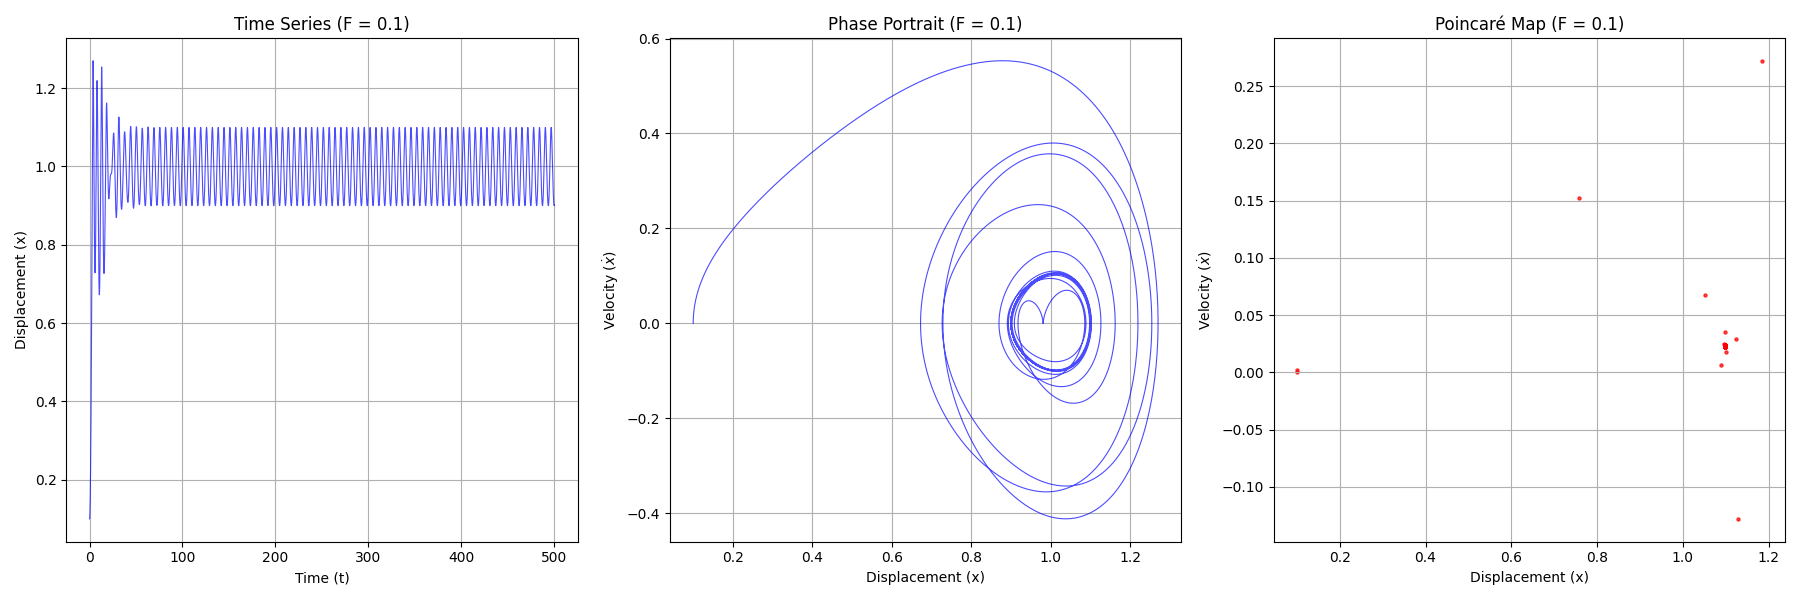
\includegraphics[width=\textwidth]{forcing_and_chaos_F_0.1.png}
    \caption{Time series, phase portrait, and Poincaré map for \(F = 0.1\). The system exhibits periodic motion.}
    \label{fig:forcing_chaos_F_0.1}
\end{figure}

\begin{figure}[h!]
    \centering
    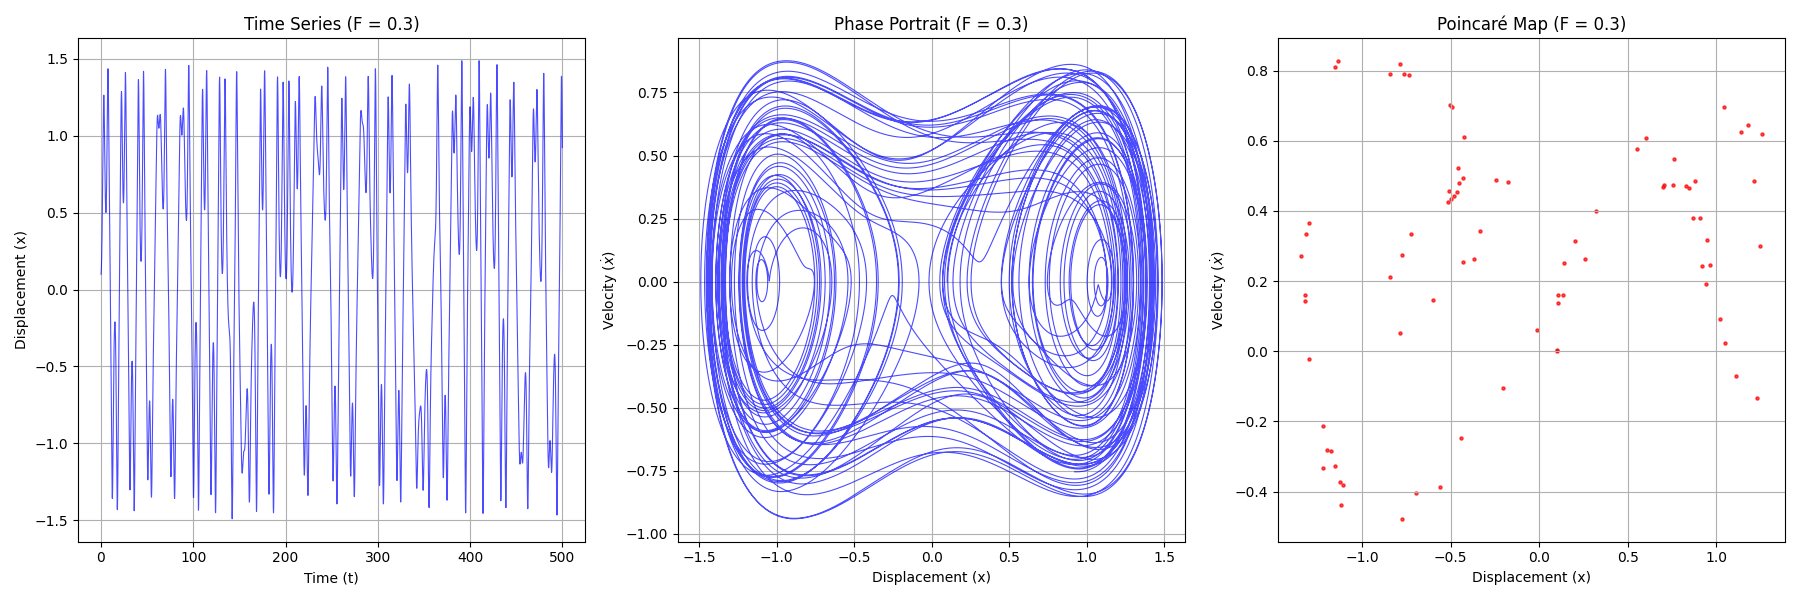
\includegraphics[width=\textwidth]{forcing_and_chaos_F_0.3.png}
    \caption{Time series, phase portrait, and Poincaré map for \(F = 0.3\). The system shows transitions to more complex dynamics.}
    \label{fig:forcing_chaos_F_0.3}
\end{figure}

\begin{figure}[h!]
    \centering
    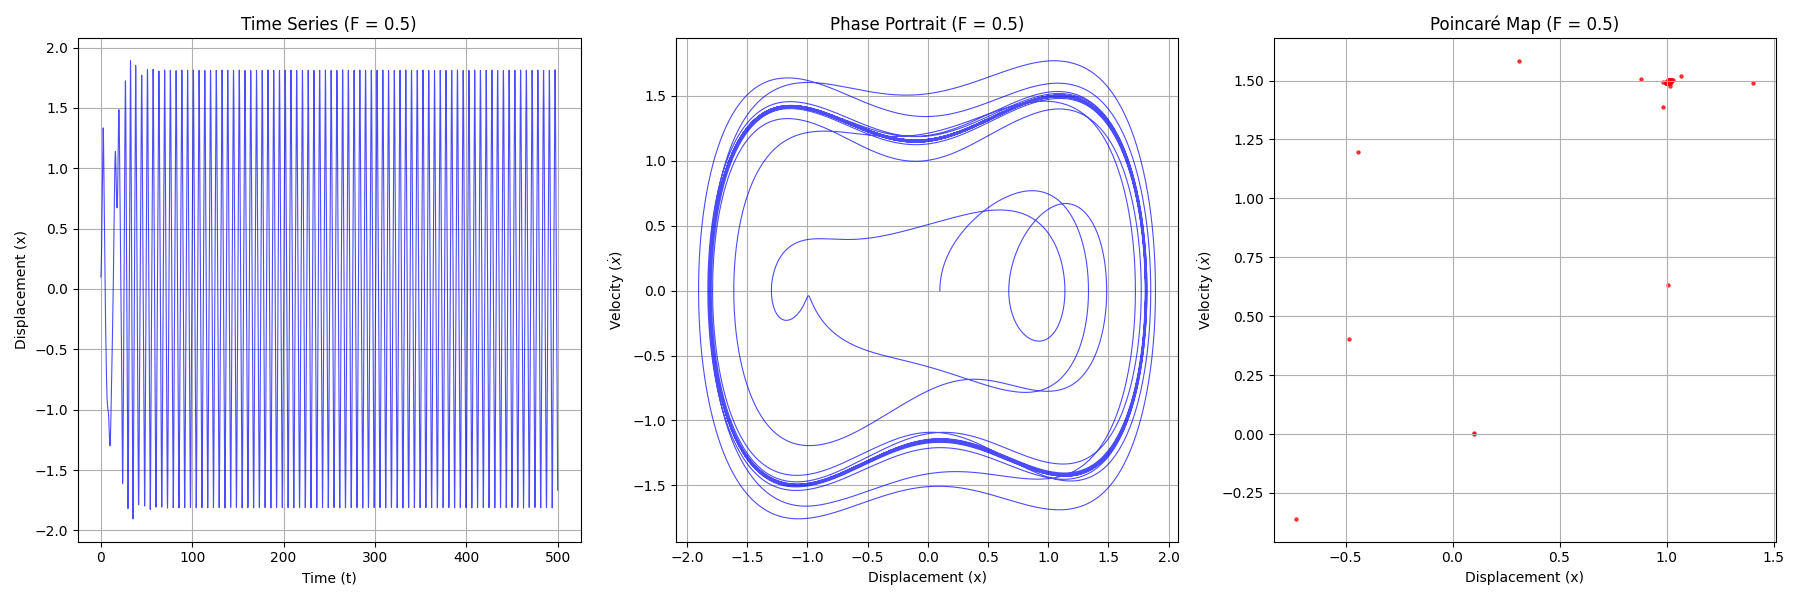
\includegraphics[width=\textwidth]{forcing_and_chaos_F_0.5.png}
    \caption{Time series, phase portrait, and Poincaré map for \(F = 0.5\). The system exhibits chaotic behavior.}
    \label{fig:forcing_chaos_F_0.5}
\end{figure}

\subsection*{Observations}
\begin{itemize}
    \item For \(F = 0.1\), the system shows periodic behavior with well-defined trajectories and Poincaré points.
    \item For \(F = 0.3\), more complex dynamics emerge, including quasiperiodic motion.
    \item For \(F = 0.5\), the system transitions to chaos, as evident from the scattered points in the Poincaré map.
\end{itemize}

\subsection*{Conclusion}
The transition from periodic motion to chaos with increasing forcing amplitude highlights the nonlinear nature of the Duffing equation and its sensitivity to parameters.

\section*{Strange Attractors}
Strange attractors are a hallmark of chaotic dynamics, representing fractal-like structures in the phase space. These attractors arise due to the sensitive dependence on initial conditions and are prominently observed in the Duffing equation under specific parameter settings.

\subsection*{Simulation and Results}
For the Duffing equation with the following parameters:
\begin{itemize}
    \item Damping coefficient: \(b = 0.2\),
    \item Linear stiffness: \(\beta = 1.0\),
    \item Forcing amplitude: \(F = 0.5\),
    \item Forcing frequency: \(\omega = 1.0\),
\end{itemize}
we observe chaotic behavior. The Poincaré map captures the structure of the strange attractor by sampling the state \((x, \dot{x})\) at multiples of the forcing period \(T = 2\pi / \omega\).

\begin{figure}[h!]
    \centering
    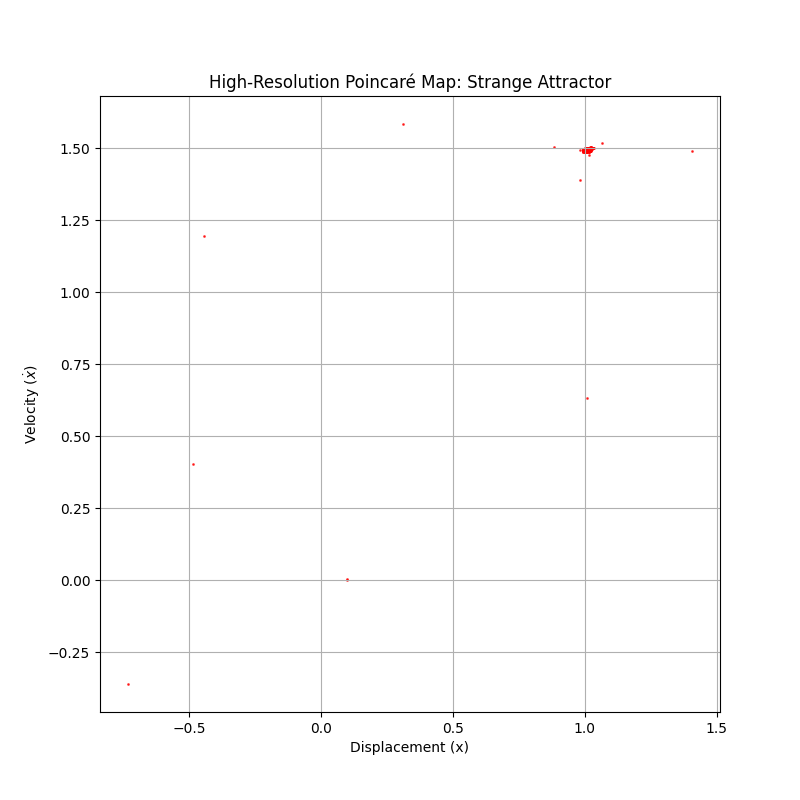
\includegraphics[width=0.8\textwidth]{strange_attractor_poincare_map.png}
    \caption{High-resolution Poincaré map showing a strange attractor for \(F = 0.5\). The fractal structure reflects the chaotic dynamics of the Duffing equation.}
    \label{fig:strange_attractor}
\end{figure}

\subsection*{Interpretation}
The strange attractor in Figure~\ref{fig:strange_attractor} exhibits:
\begin{itemize}
    \item Fractal geometry: Points in the Poincaré map do not form smooth curves but instead appear as a dense, fractal-like collection.
    \item Sensitivity to initial conditions: Small perturbations in initial conditions lead to divergent trajectories, as evidenced by the scattered points in the map.
    \item Coexistence with periodic orbits: Chaotic attractors often coexist with stable periodic orbits for certain parameter ranges.
\end{itemize}

\subsection*{Conclusion}
The strange attractor highlights the complex behavior of the Duffing equation in the chaotic regime. Its fractal structure and nonperiodic motion are key indicators of chaos, providing insights into the system's sensitivity and long-term unpredictability.

\section*{Invariant Manifolds}
Invariant manifolds describe the stable and unstable trajectories emanating from a saddle point in the phase space. These manifolds play a crucial role in understanding the transition to chaos in dynamical systems.

\subsection*{Stable and Unstable Manifolds}
For the Duffing equation:
\[
\ddot{x} + b \dot{x} - \beta x + x^3 = F \cos(\omega t),
\]
the saddle point in the phase space is located at \( (x, \dot{x}) = (0, 0) \). The stable and unstable manifolds are computed by numerically integrating the equations:
\begin{itemize}
    \item Backward in time (stable manifold): These trajectories converge to the saddle point as \(t \to \infty\).
    \item Forward in time (unstable manifold): These trajectories diverge from the saddle point as \(t \to -\infty\).
\end{itemize}

\subsection*{Simulation and Results}
Figure~\ref{fig:invariant_manifolds} shows the stable and unstable manifolds of the Duffing equation:
\begin{itemize}
    \item Blue curves: Stable manifolds, computed by integrating backward in time.
    \item Red curves: Unstable manifolds, computed by integrating forward in time.
\end{itemize}
The saddle point at \( (0, 0) \) is marked in black.

\begin{figure}[h!]
    \centering
    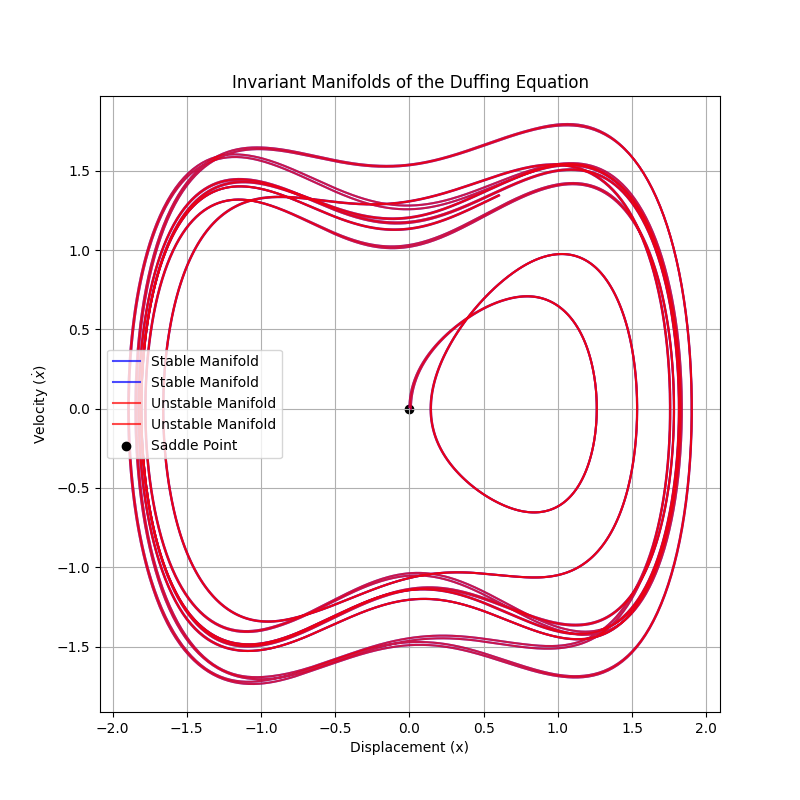
\includegraphics[width=0.8\textwidth]{invariant_manifolds.png}
    \caption{Stable and unstable manifolds of the Duffing equation. The intersections of these manifolds form homoclinic tangles, which are key indicators of chaos.}
    \label{fig:invariant_manifolds}
\end{figure}

\subsection*{Interpretation}
The manifolds exhibit the following:
\begin{itemize}
    \item The stable manifolds attract trajectories toward the saddle point.
    \item The unstable manifolds repel trajectories away from the saddle point.
    \item Their intersections form homoclinic tangles, contributing to the chaotic dynamics observed in the system.
\end{itemize}

\subsection*{Conclusion}
The invariant manifolds provide a detailed view of the phase space structure, highlighting the role of the saddle point in shaping the system's dynamics and transitions to chaos.

\section*{Bifurcation Diagram}
The bifurcation diagram visualizes the long-term dynamics of the Duffing equation as the forcing amplitude \(F\) is varied. It reveals transitions between periodic motion and chaos, showcasing the rich behavior of the system.

\subsection*{Simulation Methodology}
The Duffing equation:
\[
\ddot{x} + b \dot{x} - \beta x + x^3 = F \cos(\omega t),
\]
was simulated for \(F \in [0.1, 0.7]\), with other parameters fixed:
\begin{itemize}
    \item Damping coefficient: \(b = 0.2\),
    \item Linear stiffness: \(\beta = 1.0\),
    \item Forcing frequency: \(\omega = 1.0\).
\end{itemize}

For each \(F\), we tracked the displacement \(x\) at regular intervals corresponding to the forcing period \(T = 2\pi/\omega\), after discarding the transient dynamics. The resulting points were plotted against \(F\) to construct the bifurcation diagram.

\subsection*{Results}
Figure~\ref{fig:bifurcation_diagram} shows the bifurcation diagram:
\begin{figure}[h!]
    \centering
    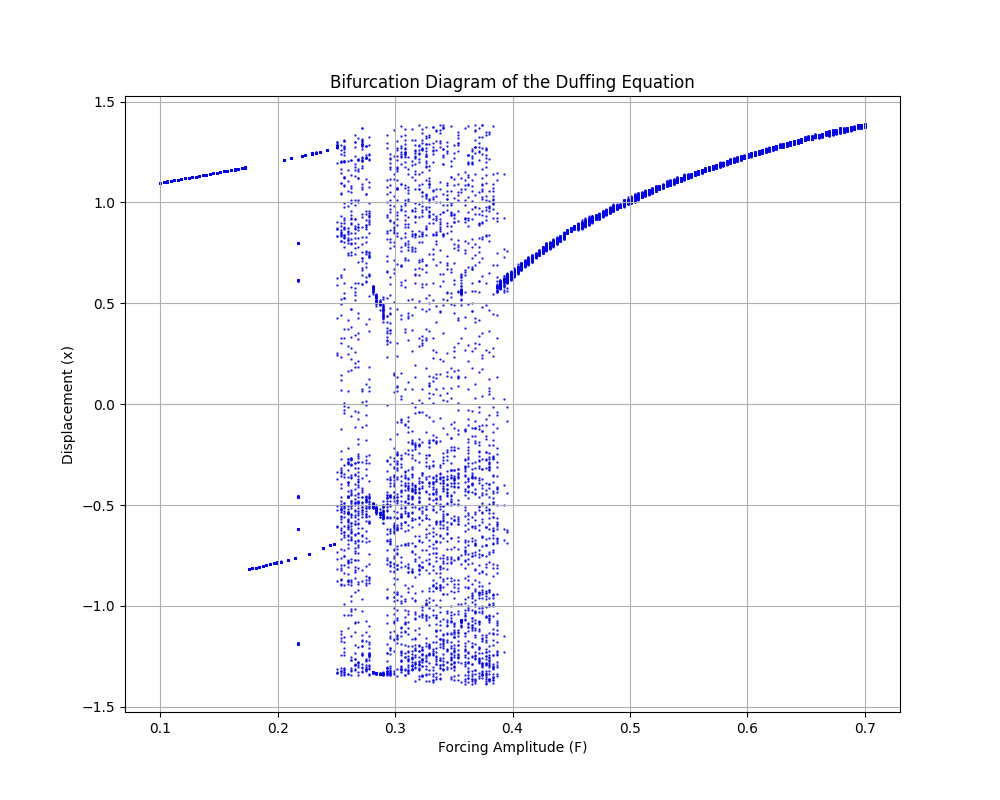
\includegraphics[width=0.8\textwidth]{bifurcation_diagram.png}
    \caption{Bifurcation diagram of the Duffing equation. The diagram illustrates transitions from periodic motion to chaos as \(F\) increases.}
    \label{fig:bifurcation_diagram}
\end{figure}

\subsection*{Observations}
The bifurcation diagram reveals:
\begin{itemize}
    \item For small \(F\), the system exhibits periodic motion, evident from single points or small clusters.
    \item As \(F\) increases, period-doubling cascades are observed, with the number of points doubling at each bifurcation.
    \item At higher \(F\), chaotic motion emerges, characterized by dense, scattered points.
    \item Periodic windows within chaotic regimes can also be observed for specific \(F\) values.
\end{itemize}

\subsection*{Conclusion}
The bifurcation diagram highlights the nonlinear behavior of the Duffing equation, showcasing its transitions between order and chaos. These transitions are a hallmark of complex dynamical systems.

\section*{Power Spectrum Analysis}
The power spectrum provides a frequency-domain representation of the Duffing equation's motion, highlighting the dominant frequencies and their amplitudes. It is particularly useful for distinguishing between periodic and chaotic dynamics.

\subsection*{Simulation and Results}
The Duffing equation:
\[
\ddot{x} + b \dot{x} - \beta x + x^3 = F \cos(\omega t),
\]
was simulated with the following parameters:
\begin{itemize}
    \item Damping coefficient: \(b = 0.2\),
    \item Linear stiffness: \(\beta = 1.0\),
    \item Forcing amplitude: \(F = 0.5\),
    \item Forcing frequency: \(\omega = 1.0\).
\end{itemize}

The displacement \(x(t)\) was transformed into the frequency domain using the Fast Fourier Transform (FFT), and the power spectrum was computed as:
\[
P(f) = |\mathcal{F}[x(t)]|^2,
\]
where \(f\) is the frequency and \(\mathcal{F}[x(t)]\) is the Fourier transform of \(x(t)\).

\subsection*{Results}
Figure~\ref{fig:power_spectrum} shows the power spectrum of the Duffing equation's motion:
\begin{figure}[h!]
    \centering
    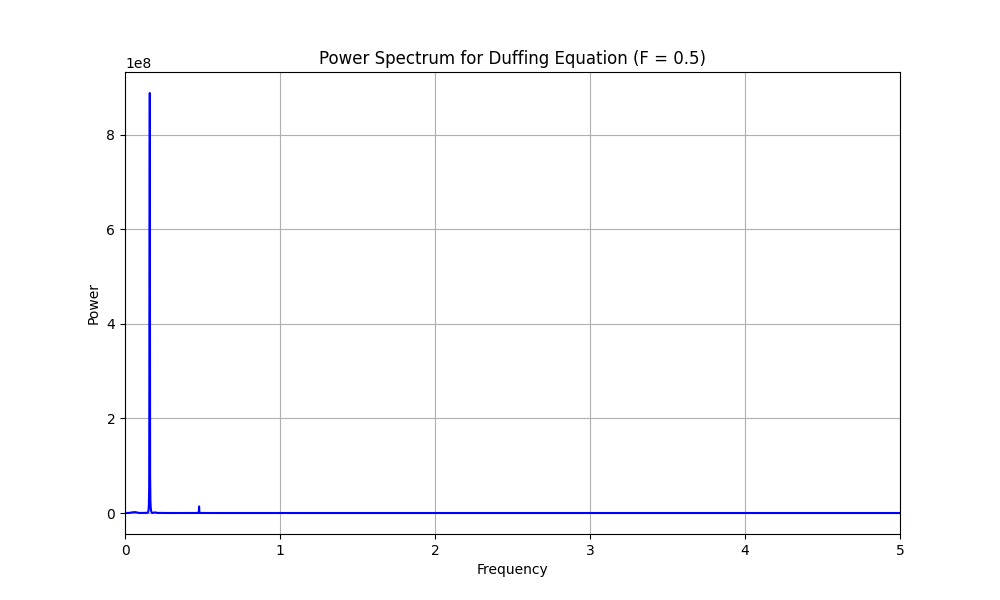
\includegraphics[width=0.8\textwidth]{power_spectrum.png}
    \caption{Power spectrum of the Duffing equation for \(F = 0.5\). The broad spectrum indicates chaotic behavior, with dominant peaks corresponding to the forcing frequency and its harmonics.}
    \label{fig:power_spectrum}
\end{figure}

\subsection*{Observations}
The power spectrum reveals:
\begin{itemize}
    \item Dominant peaks at the forcing frequency (\(\omega = 1.0\)) and its harmonics, corresponding to periodic components.
    \item A broad spectrum, characteristic of chaotic dynamics, indicating the presence of multiple interacting frequencies.
\end{itemize}

\subsection*{Conclusion}
The power spectrum provides a detailed view of the system's dynamics in the frequency domain. Periodic behavior manifests as sharp peaks, while chaotic dynamics produce a broad, noisy spectrum with dominant frequencies still identifiable.


\end{document}
